\chapter{Learning and Testing from Real-World Data}

Enumerative inference on synthetic traces can provide low-level confirmation about basic properties of our model, under simple qualitative conditions.
However, real-world analysis provides a much richer set of possibilities in terms of analyzing and improving our model.
We collect a set of real-world videos containing common household items from the YCB object dataset, along with annotated values for all of the variables in the static (single frame) version of our model.
We then use this data in a gradient search to train a subset of hyperparameters that have thus far been hand-selected through trial-and-error, but may not be properly tuned to model real-world data.
We also measure the performance of our proposed structure inference algorithm on predicting the ground-truth structure from a set of object poses.

\section{Data Specification}
We collect a set of experiments with static objects to analyze the model in the static case.
We add noise via occluders that temporarily block the camera's line of sight to the objects.
The raw video was collected using the Intel RealSense D435 RGB/Depth camera.
Only the RGB information is used for the neural detector, but we collect depth data to enable plane detection, and for future tests on models containing likelihood over depth data.
Observed poses are generated using the publicly provided nVidia DOPE detector GitHub repository.
Ground truth outlier status is manually annotated for each frame in the collected videos.
Note that using the vertices, we can also use the scene graph structure to determine which detections are false positives or negatives.

Ground truth structure is manually annotated once per scene, and the ground truth poses are estimated as the average over all an object's detected \textit{inlier} poses.
While this obscures systematic bias across all neural detections in the data set, in nonetheless provides a useful relative analysis of the stability of the neural detector in the presence of varying levels of occlusion.
This data set generation process is easily scalable, as all it requires manually is the collection of the video, a once-per-scene annotation of the static ground truth structure, and a per-frame annotation of which neural detections were decently well-localized inliers.
Table~\ref{table:inhouseDatasetSpec} lists the data collected for each scene, while Figure~\ref{fig:inhouseDataset} shows some representative samples from our data set.

\begin{table}[H]
\begin{tabular}{|p{2.5cm}|p{4cm}|p{7.5cm}|}
\hline
\textbf{Name}               & \textbf{Data}          & \textbf{Description} \\
\hline
\textit{Observed poses}              & (String, List[Pose]) & nVidia Deep Object Pose Estimator neural detections \\
\hline
\textit{Ground truth outlier status} & (String, List[Bool]) & Per-Frame, per-object flag indicating if an object's neurally generated pose estimate is a noisy outlier \\
\hline
\textit{Ground truth scene graph}    & Scene Graph          & Observed static structure, and object poses estimated as the average of inlier detections. \\
\hline
\end{tabular}
\caption{Description of data collected in our real-world experiments with YCB objects.}
\label{table:inhouseDatasetSpec}
\end{table}

\begin{figure}[H]
  \begin{subfigure}[b]{0.72\textwidth}
    \centering
    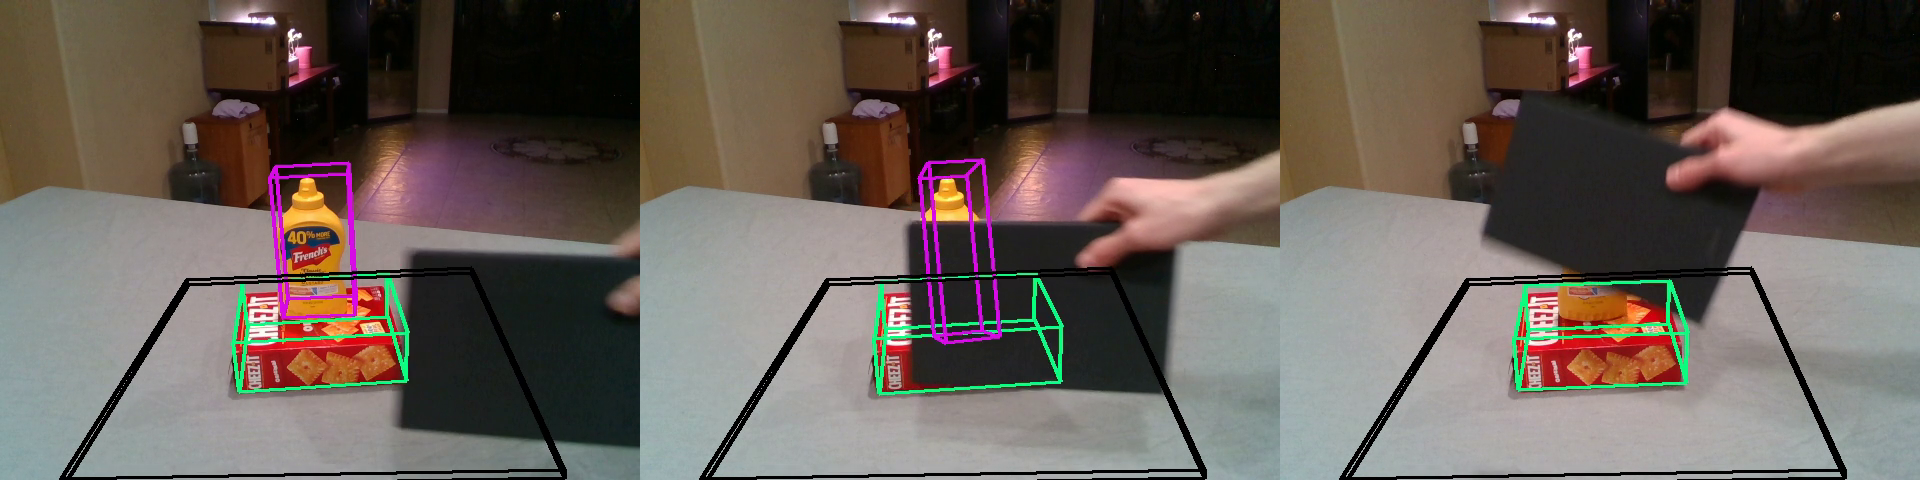
\includegraphics[width=\columnwidth]{inhouseDataset1}
  \end{subfigure}%
  \hspace{0.3cm}
  \begin{subfigure}[b]{0.24\textwidth}
    \centering
    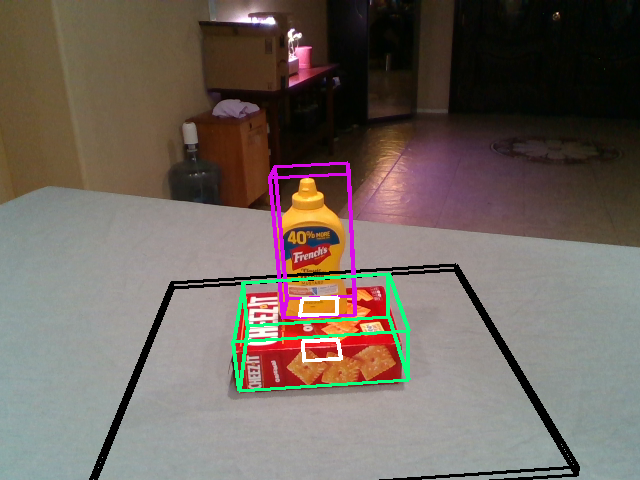
\includegraphics[width=\columnwidth]{inhouseGroundTruth1}
  \end{subfigure}
  \vspace{0.1cm}

  \begin{subfigure}[b]{0.72\textwidth}
    \centering
    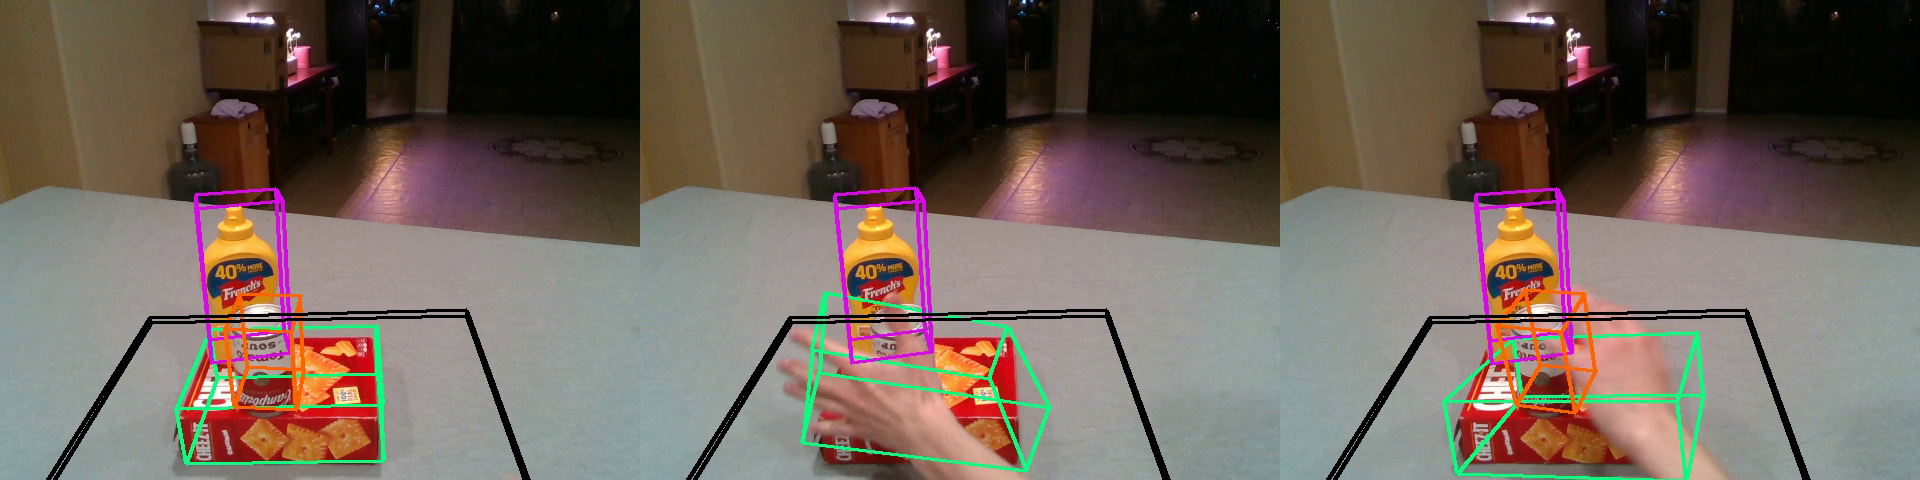
\includegraphics[width=\columnwidth]{inhouseDataset4}
  \end{subfigure}%
  \hspace{0.3cm}
  \begin{subfigure}[b]{0.24\textwidth}
    \centering
    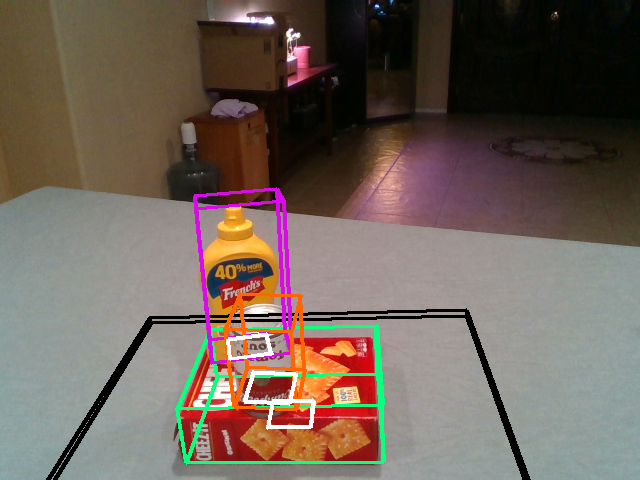
\includegraphics[width=\columnwidth]{inhouseGroundTruth4}
  \end{subfigure}
  \vspace{0.1cm}

  \begin{subfigure}[b]{0.72\textwidth}
    \centering
    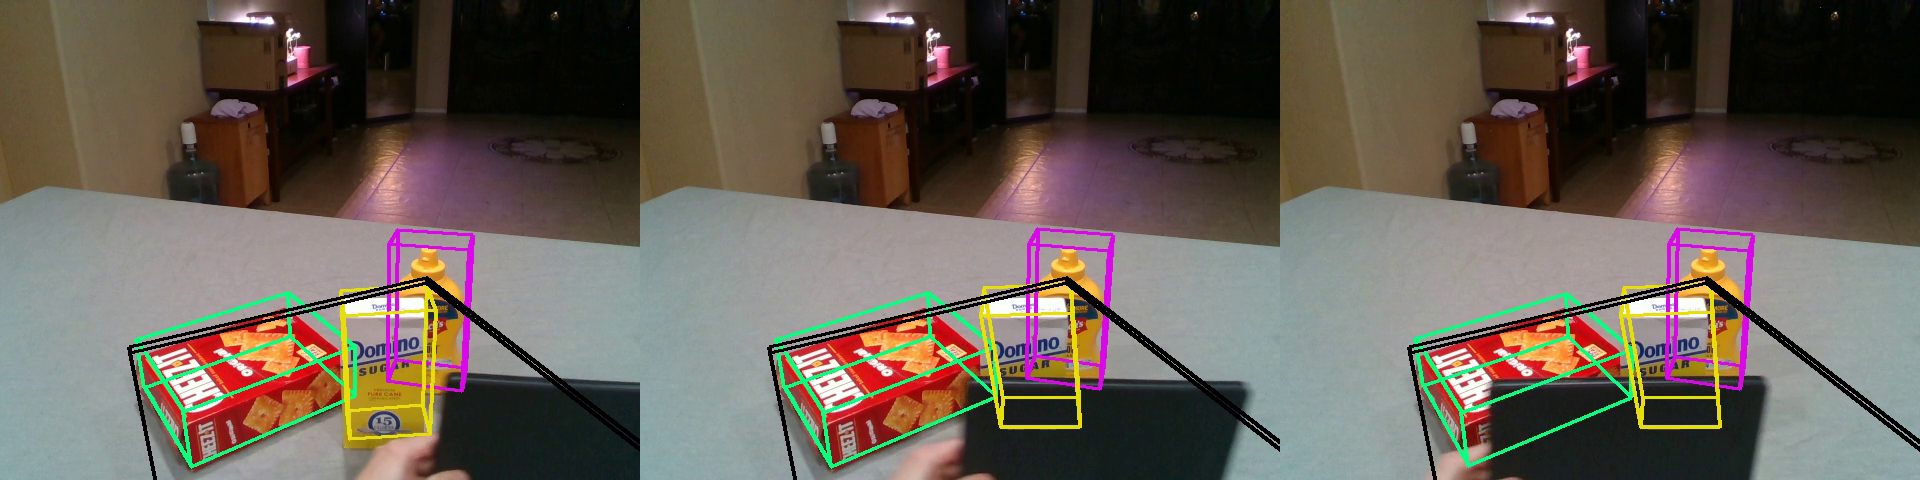
\includegraphics[width=\columnwidth]{inhouseDataset5}
  \end{subfigure}%
  \hspace{0.3cm}
  \begin{subfigure}[b]{0.24\textwidth}
    \centering
    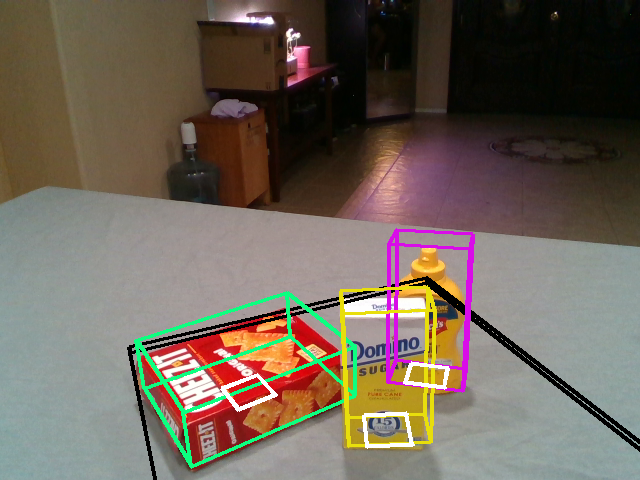
\includegraphics[width=\columnwidth]{inhouseGroundTruth5}
  \end{subfigure}
  \vspace{0.1cm}

  \begin{subfigure}[b]{0.72\textwidth}
    \centering
    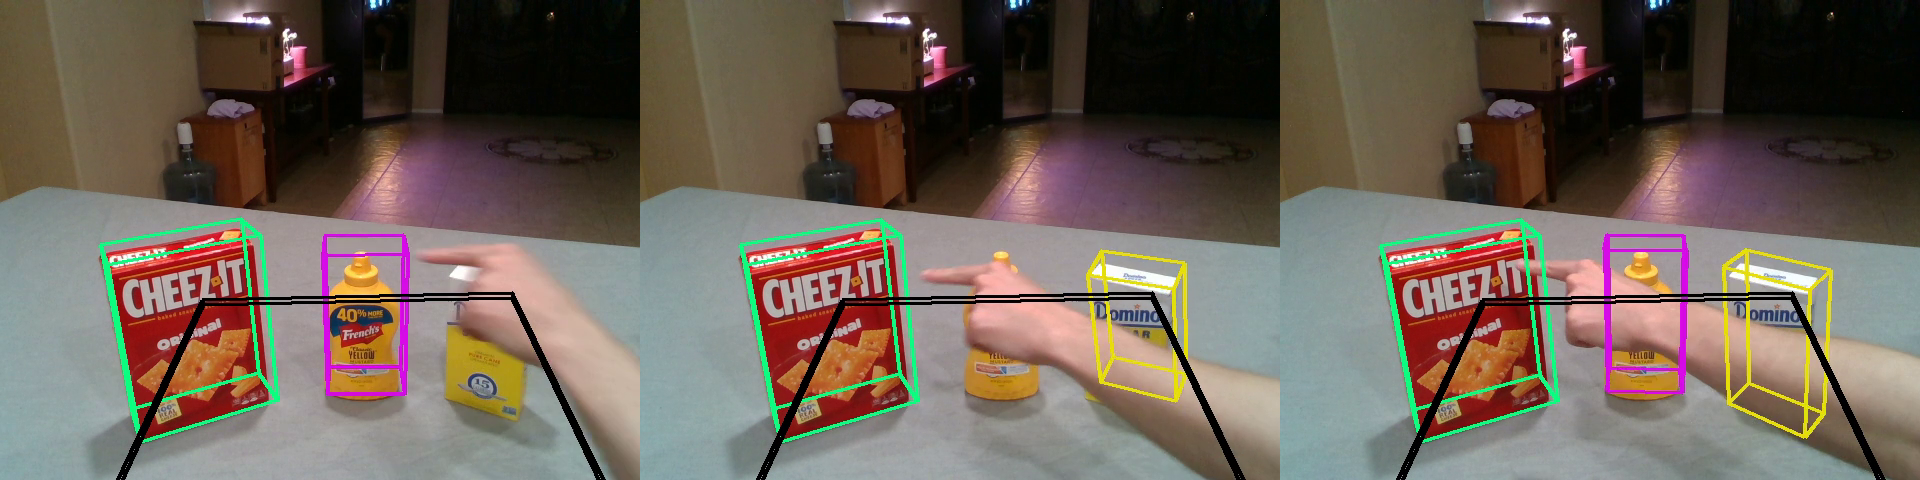
\includegraphics[width=\columnwidth]{inhouseDataset6}
  \end{subfigure}%
  \hspace{0.3cm}
  \begin{subfigure}[b]{0.24\textwidth}
    \centering
    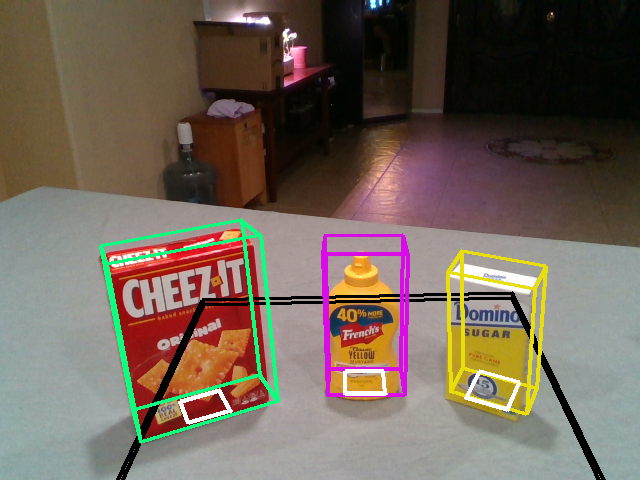
\includegraphics[width=\columnwidth]{inhouseGroundTruth6}
  \end{subfigure}
  \vspace{0.1cm}

  \begin{subfigure}[b]{0.72\textwidth}
    \centering
    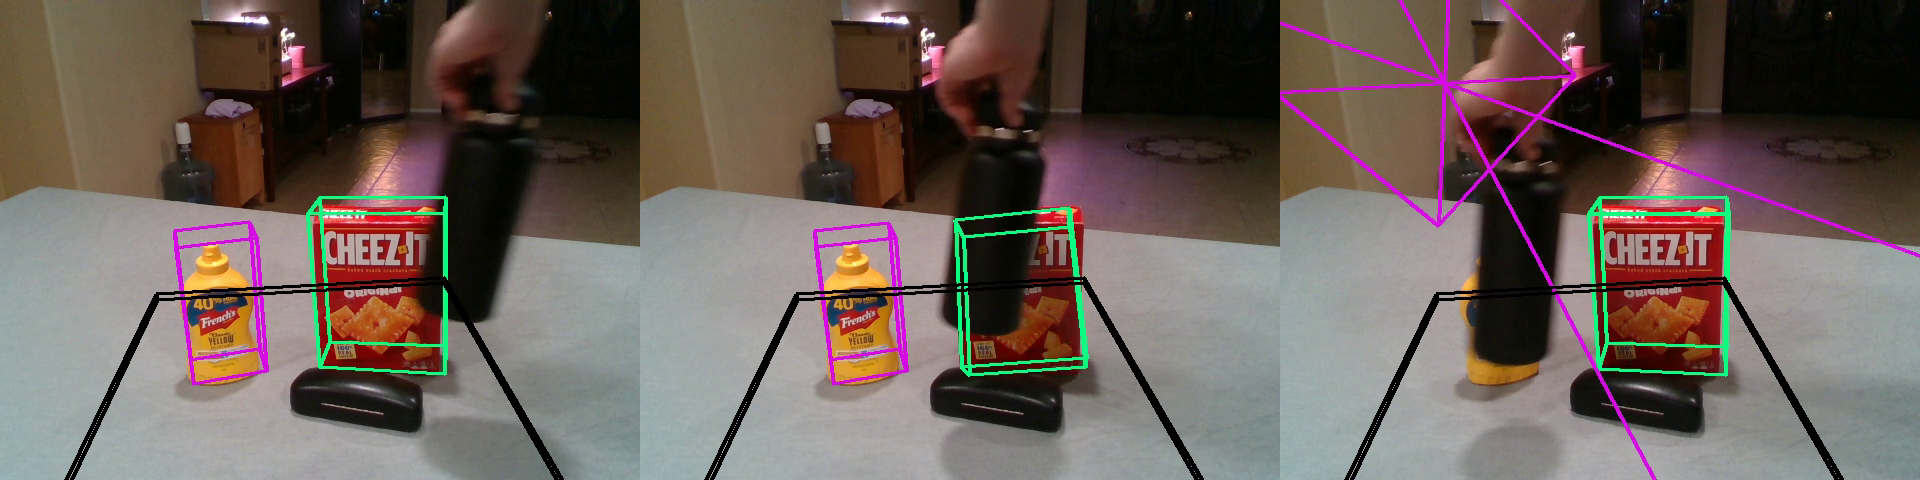
\includegraphics[width=\columnwidth]{inhouseDataset8}
  \end{subfigure}%
  \hspace{0.3cm}
  \begin{subfigure}[b]{0.24\textwidth}
    \centering
    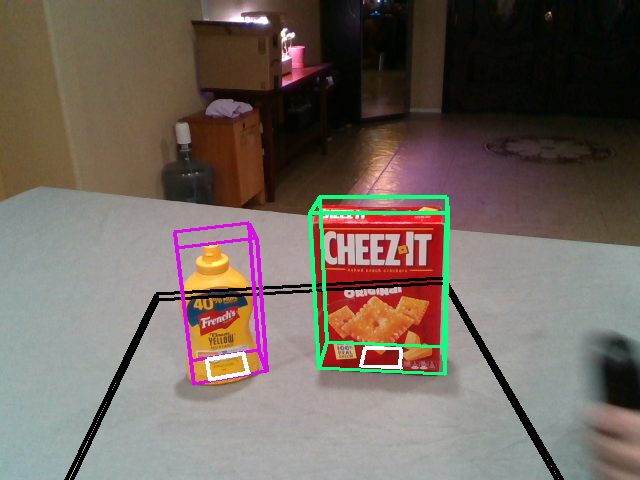
\includegraphics[width=\columnwidth]{inhouseGroundTruth8}
  \end{subfigure}
  \vspace{0.1cm}

  \caption{
    A selection of frames from 5 of the 8 captured videos.
    (Left) We use a dynamic occluder to generate noise in the observed neural network detections, in which objects have their poses estimated incorrectly, or even flicker out of existence.
    (Right) Each scene is represented by a single static scene graph, with manually annotated structure, and object poses estimated as the average of the inlier neural detections.
  }
  \label{fig:inhouseDataset}
\end{figure}

\pagebreak

\section{Metrics}
\subsection{Modeling: Marginal Likelihood}
The most immediate metric measuring the evidence for our model given the data is the log likelihood.
Since we've collected complete data for our model, the likelihood simply ends up being the joint probability density of the trace.
In Gen, given a collection of traces $t \in \mathcal{T}$ and hyperparameters $\theta$, the log-likelihood is:
\[
  \ell(\mathcal{T}; \theta) = \sum_{t \in \mathcal{T}} \log p(t_i; \theta)
\]

\subsection{Structure Inference: Graph Edit Distance}
When evaluating the performance of structure inference, we would like a measure of the similiary of the most probable inferred structure to the ground truth.
This gives a measure of how far our algorithm is from ground truth when tasked with classifying the structure of an unambiguous scene.
In particular, we simplify our metric to how well our algorithm correctly determines which objects in a scene are ``contacting''.
To do this, we reduce the structure of the predicted scene graph $G_1$ and target scene graph $G_2$ to a simple set of undirected edges.
The graph operations we consider ``edits'' are edge addition and edge removal.
Then, the edit distance is just the size of the symmetric distance $E_1 \triangle E_2$ of the edge sets, or more explicitly
\[
  \mathrm{Edit}(E_1, E_2) = \abs{E_1 \triangle E_2} = \abs{(E_1 \cup E_2) \setminus (E_1 \cap E_2)}
\]

\section{Learning Hyperparameters with Gradient Ascent}
We can perform a data-driven maximum, we can now use gradient-based optimization to automatically tune the static model hyperparameters to our data, and measure the increase in log-likelihood.
We select 3 hyperparamters $\bm{\sigma} = (\sigma_1, \sigma_2, \sigma_3)$ to optimize over: the standard deviation $\sigma_1 = \sigma_\mathrm{inlier}$ for the observed 3D positions, the standard deviation $\sigma_2 = \sigma_\mathrm{slack}$ for the 1D slack offsets, and the standard deviation $\sigma_3 = \sigma_\mathrm{sliding XY}$ for the latent $(x,y)$ contact parameters.
We'd like to find
\[
  \max \ell(\mathcal{T}; \bm{\sigma}) = \sum_{t \in \mathcal{T}} \log\ p(t; \bm{\sigma})
\]

To do so, we perform a scheduled gradient ascent over the hyperparameters with respect to the objective function.
We initialize $\bm{\sigma}_0 = (0.01, 0.01, 0.25)$ (meters).
We run 1,000 iterations of gradient descent, and for each iteration $t$ we update parameters according to
\[
  \bm{\sigma}_t = \bm{\sigma}_{t-1} + \alpha_0 r^{t} \cdot \nabla\bm{\sigma}_{t-1}
\]

where $\alpha_0 = \num{1e-8}$ and $r = 0.999$.
Gen's dynamic DSL supports automatic calculation of gradients of the joint density evaluated on the conditioned addresses, with respect to model hyperparameters, and for performing updates on parameters with a provided learning rate.
Thus our procedure is mostly automated once we have the set of traces $\mathcal{T}$.

Figure~\ref{fig:hyperparamGD} shows the results of gradient descent.
The algorithm converges rather rapidly for $\sigma_\mathrm{inlier}$ and $\sigma_\mathrm{slack}$, but over a longer time we see $\sigma_\mathrm{sliding XY}$ begin to converge as well.
This longer convergence time suggests that $\sigma_\mathrm{sliding XY}$ may have a smaller impact overall on the likelihood compared to the other two parameters.

\raggedbottom
\pagebreak
\flushbottom

\begin{figure}[H]
  \centering
  \begin{subfigure}[b]{0.75\textwidth}
    \centering
    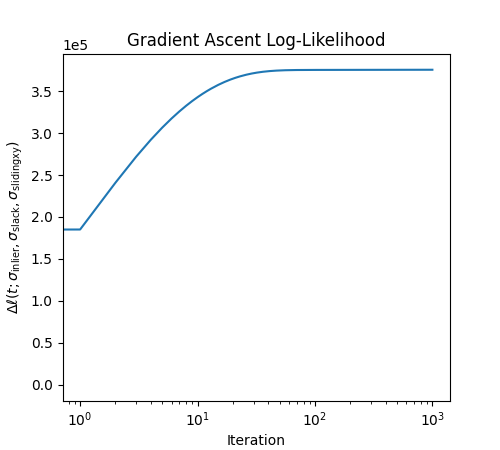
\includegraphics[width=\columnwidth]{hyperparamGDObjective}
  \end{subfigure}
  \begin{subfigure}[b]{0.75\textwidth}
    \centering
    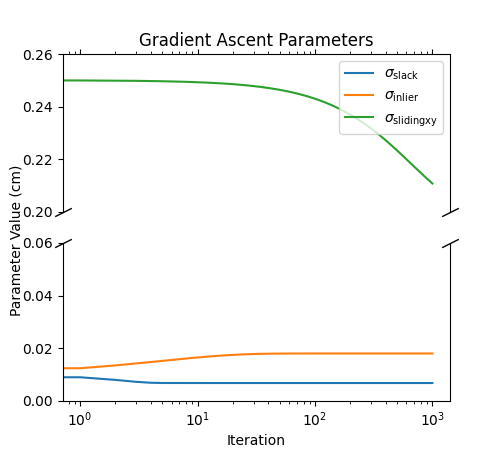
\includegraphics[width=\columnwidth]{hyperparamGDParams}
  \end{subfigure}
  \caption{
    Results of gradient ascent on $\bm{\sigma}$.
    (Top) shows the change in log likelihood $\Delta\ell(\mathcal{T}; \bm{\sigma}) = \ell(\mathcal{T}; \bm{\sigma}_t) - \ell(\mathcal{T}; \bm{\sigma}_0)$.
    (Bottom) shows the values of the parameters $\bm{\sigma}_t$.
  }
  \label{fig:hyperparamGD}
\end{figure}


\section{Inlier Detection Observational Model}
\begin{figure}[H]
  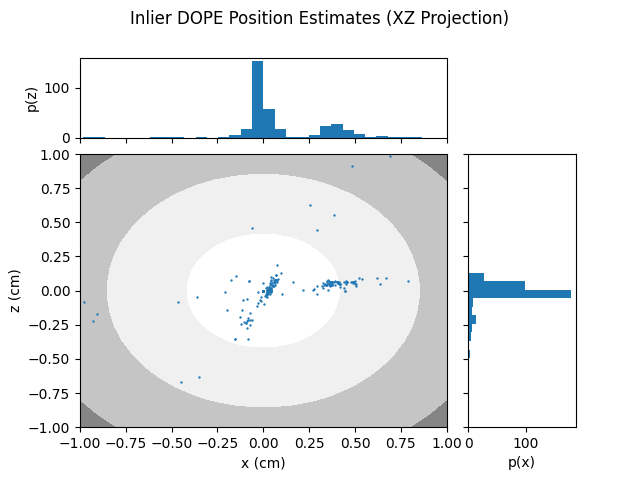
\includegraphics{topdownInlierDetections}
  \caption{
    Scatter plot of the projection of nVidia DOPE's observed pose estimates to the x and z position axes, along with corresponding marginal histograms for each axis respectively.
    The plotted contour is the overlaid noisy observation model for inlier detections (in the projection, a 2D multivariate normal distribution), with the standard deviation hyperparameter set to the maximum-likelihood value for $\sigma_\mathrm{slack}$ that we optimized for above.
  }
  \label{fig:topdownInlierDetections}
\end{figure}
The lowest-level data in our static model are observations of neural object detections.
A-priori, we modeled this data as a simple mixture of an ``inlier'' and ``outlier'' distribution.
We presupposed the noise for detected inlier positions would be normally distributed, with standard deviation $\sigma_\mathrm{slack}$.
In the last section, we jointly fit this hyperparameter with two others, which gives us a tuned version of our inlier model.

Figure~\ref{fig:topdownInlierDetections} provides a comparison of a simple observational model in the positional dimensions, fit to maximum likelihood with respect to inlier pose detections.
We note a few details from this plot, and what they suggest for the observational model.

The first is that the distribution systematically overestimates the number of observations in the ``middle'' part of the space.
A large number of detected poses are either highly concentrated around the mean detection, or are much further out in the tails of the distribution.
A normal distribution may not be the most accurate model of the behavior of the neural detector; a distribution with heavier tails, such as a Cauchy, is likely to better model of the detected positions.

The second is the presence of ``clusters'' of erroneous detections that suggest failures in the neural detectors are strongly correlated across time.
Indeed, the high concentration of poses around the average inlier detection means that there could be substantial correlated systematic error in an object's detection across an entire scene, that is not shown in Figure~\ref{fig:topdownInlierDetections}.
For example, the average inlier pose detection for the Domino sugar box presented on the right side of the fourth row in Figure~\ref{fig:inhouseDataset} is visibly mis-estimated.
Assuming that observational noise is falsely uncorrelated can bias our posterior latent pose to be centered around a systematically wrong detection.
It may instead be possible to model the correlation between these errors, and use additional information from the image, like the presence of occluders, to obtain a more accurate estimate of the true object pose.

\raggedbottom
\pagebreak
\flushbottom

\section{Testing Structure Inference}
\begin{figure}[H]
  \begin{subfigure}[b]{\textwidth}
    \centering
    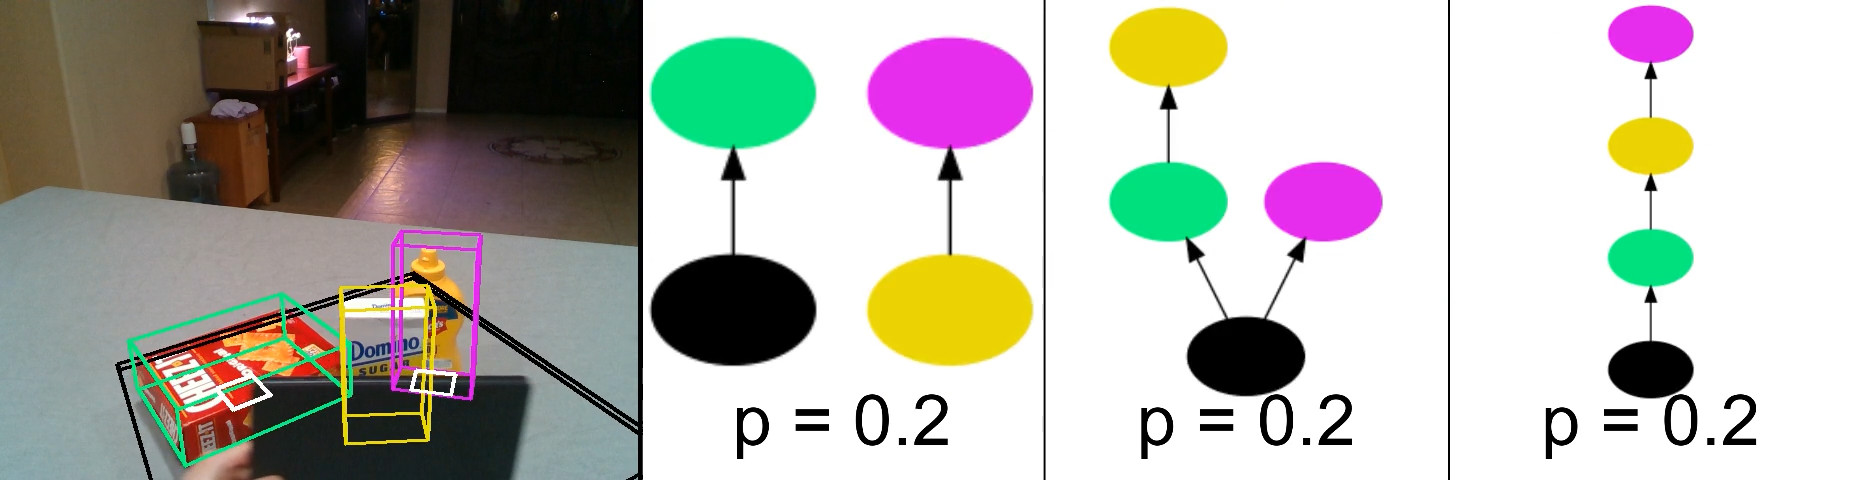
\includegraphics[width=\columnwidth]{rjmcmcBefore}
  \end{subfigure}
  \begin{subfigure}[b]{\textwidth}
    \centering
    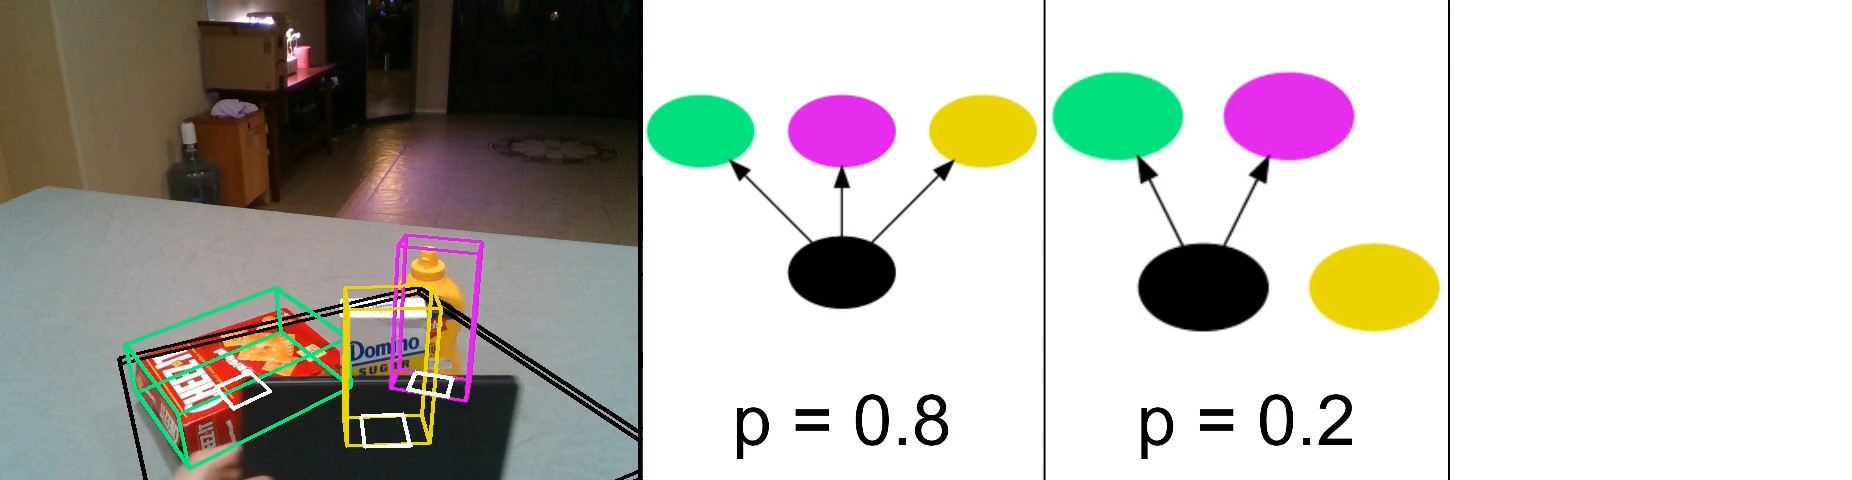
\includegraphics[width=\columnwidth]{rjmcmcAfter}
  \end{subfigure}
  \label{fig:rjmcmcExample}
  \caption{
    Example of the performance on RJMCMC on inferring the structure posterior in a frame from scene \#5.
    (Top) The uniform prior over scene graph structure contains a random assortment of inaccurate classifications.
    (Bottom) The RJMCMC structure inference procedure predicts the correct ground-truth structure with high probability.
  }
\end{figure}
Finally, we use our real-world data to evaluate the performance of our RJMCMC procedure for structure inference, on the posterior for our unoptimized and optimized models.
We want to see how well our procedure is able to classify the ground truth structure, given the correct latent poses of the objects in a scene.
However, we only have the ground truth poses for 8 unique static scenes, which limits the number of independent trials we can perform.

To ameliorate this, we augment the data with some sampled noise.
When performing continuous parameter inference our latent pose posterior will have some non-zero width, meaning we should allow for some variability in the estimated underlying pose, without significantly changing the structure posterior.
To simulate this, we augment our data by very slightly perturbing the latent poses for each frame, without qualitatively changing the underlying scene graph that best explains these latent poses; the position is perturbed by gaussian noise sampled with a standard deviation of 0.5 cm, and the orientation is perturbed by VMF noise sampled with concentration parameter 4000.
This adds enough variability to give a more robust test of our structure inference algorithm, especially when comparing the unoptimized and optimized models.

For each frame, we set the static model trace to the underlying scene graph in 5 independent particles.
For each particle, we then resample the scene graph structure $G$ and discrete parameters $Z$ from a uniform prior, without changing the absolute 6DoF poses or observations for each object.
We then sweep our reversible jump structure move across all objects $O$ for 5 iterations.
Figure~\ref{fig:rjmcmcResults} shows the graph edit distance between the ground-truth structure and the most frequent structure among the particles, in the unoptimized and optimized case respectively.
Figure~\ref{fig:rjmcmcExample} shows an example of the prior structure and inferred posterior respectively for a frame in sequence \#5.
Inference in both cases consistently finds a structure within two edges of the ground-truth, and most often finds the correct structure.

The optimized procedure performs marginally better than the unoptimized case, although the difference is minimal.
Given this, and the fact that our hyperparameters didn't change much in the gradient ascent procedure, suggests that our hand-tuned values were already decent to begin with, at least with respect to the structure posterior.
Recall that in our synthetic analysis of these hyperparameters shown in Figure~\ref{fig:posStructurePosterior}, the posterior probability of an edge between two objects transitions rather sharply between 0 and 1, depending on the distance of their contacting faces.
We might then expect that for a range of ``decently-tuned'' hyperparameter values, the structure posterior would perform roughly the same, with a sharp decrease in model performance once the hyperparmeters fell out of this range.

\begin{figure}[H]
  \centering
  \begin{subfigure}[b]{0.75\textwidth}
    \centering
    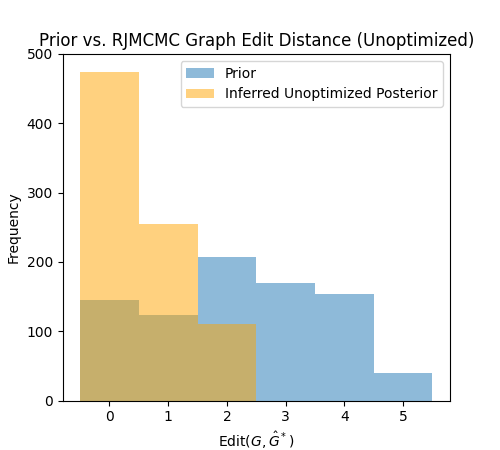
\includegraphics[width=\columnwidth]{rjmcmcUnoptimized}
  \end{subfigure}
  \begin{subfigure}[b]{0.75\textwidth}
    \centering
    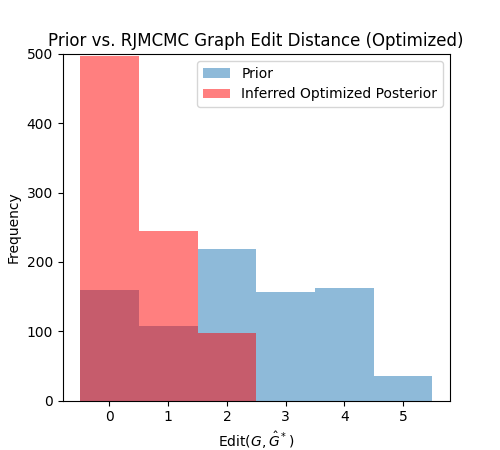
\includegraphics[width=\columnwidth]{rjmcmcOptimized}
  \end{subfigure}
  \caption{
    Graph edit distance between the ground truth structure $G$ and the mode $\hat{G}^*$ of the inferred structure posterior, for the unoptimized model (top) and optimized model (bottom).
  }
  \label{fig:rjmcmcResults}
\end{figure}
